\documentclass{article}
\usepackage{graphicx}
\usepackage{geometry}
\geometry{a4paper, margin=1in}

\title{Optimized Wing Design Report}
\author{LLM Assistant}
\date{2025-06-08}

\begin{document}
\maketitle

\section{Executive Summary}
This report summarizes the optimization process for a wing design with the objective of minimizing drag at a lift coefficient (CL) of 2.0, a wing area (S) of 100 m$^2$, and a span (b) of 10 m. The design variables included taper, twist, and sweep. The optimization was performed using the ScipyOptimizeDriver with the SLSQP algorithm. The optimization process concluded with a 'FAIL' status after 183 iterations, indicating a non-optimal solution. The resulting drag coefficient (CD) is 0.118, which is considered high.

\section{Analysis of Results}

As indicated by the 'FAIL' status, the optimization did not converge to an optimal solution. The solver terminated prematurely, potentially due to getting stuck in local minima or the problem's complexity exceeding the algorithm's capabilities. The optimized wing geometry, visualized in Figure \ref{fig:optimized_wing}, shows the wing design at iteration 182. The lift distribution deviates significantly from the ideal elliptical lift distribution, which is known to minimize induced drag. Additionally, the twist distribution plot appears to have stalled at its upper bound, suggesting that the bounds may be overly restrictive.

\begin{figure}[h!]
    \centering
    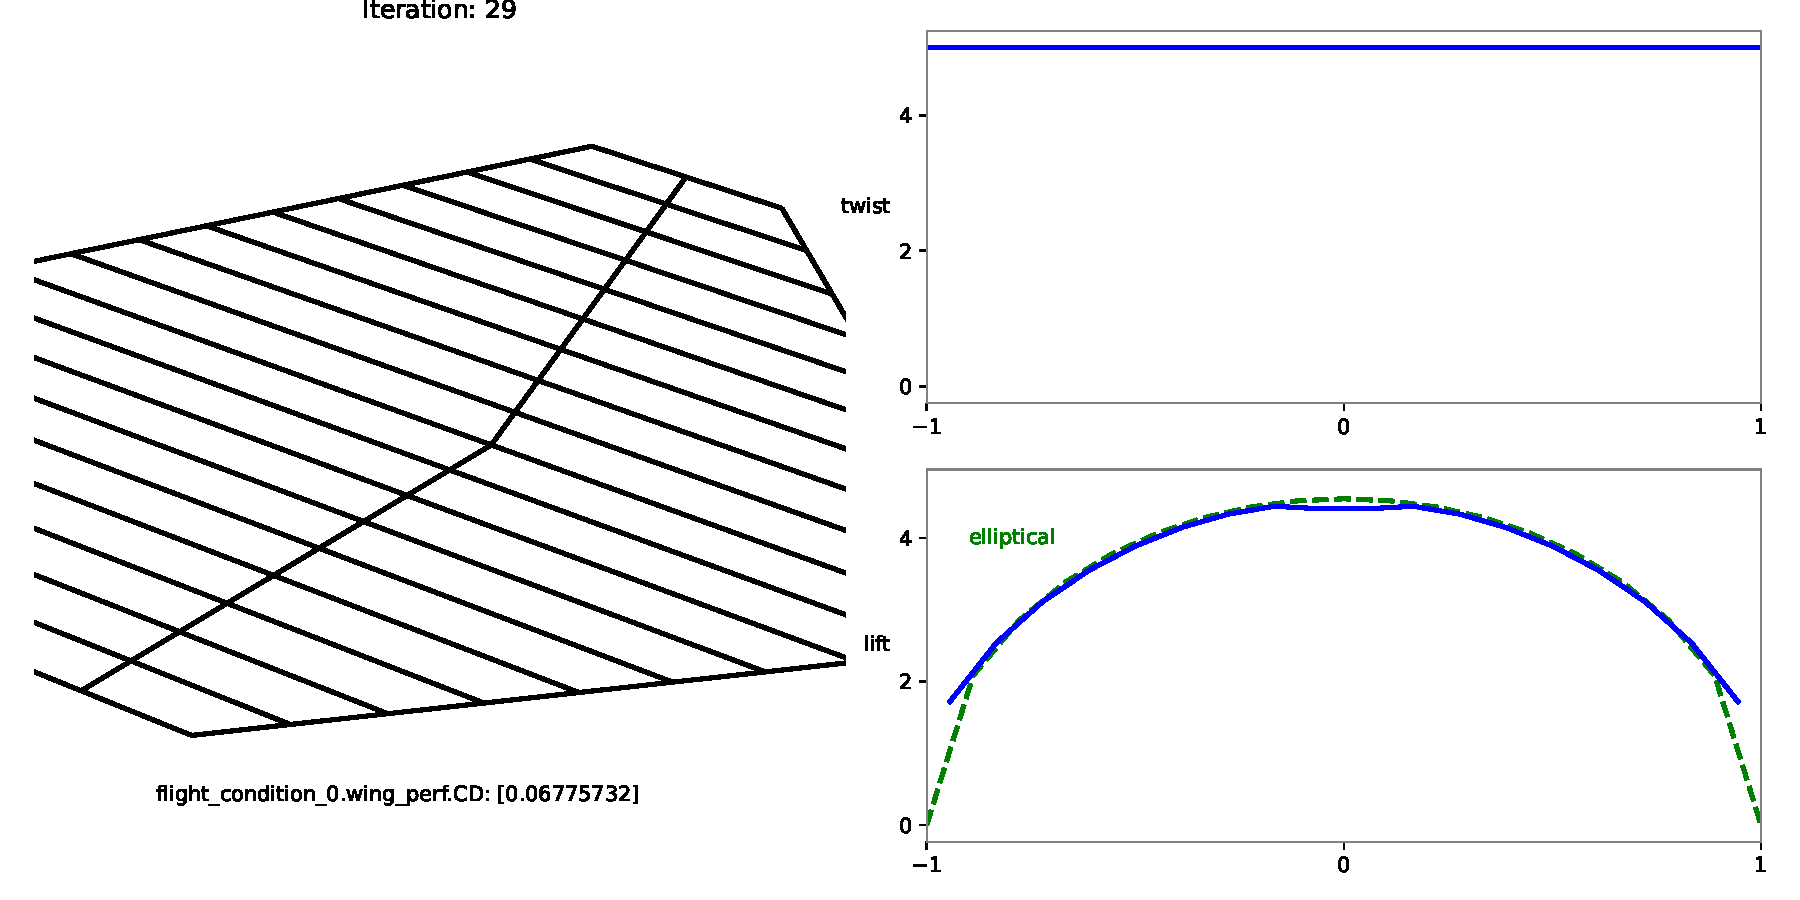
\includegraphics[width=0.7\textwidth]{./Optimized_Wing.pdf}
    \caption{Optimized Wing Visualization at Iteration 182}
    \label{fig:optimized_wing}
\end{figure}

The optimization process involved 183 model evaluations and 28 derivative evaluations, with a wall clock run time of approximately 3.4 seconds. The high drag coefficient and the 'FAIL' status suggest that the SLSQP algorithm struggled to efficiently handle the problem's complexity.

\section{Recommendations}

To improve the optimization process and achieve a more optimal wing design, the following recommendations are proposed:

\begin{enumerate}
    \item \textbf{Investigate the cause of the 'FAIL' status:} Analyze the optimization log and error messages to understand the reason for premature termination.
    \item \textbf{Adjust optimization settings:} Increase the maximum number of iterations (\texttt{maxiter}) and consider reducing the tolerance to allow for finer convergence.
    \item \textbf{Try different optimization algorithms:} Explore alternative gradient-based algorithms like BFGS or CG, or gradient-free algorithms such as genetic algorithms or simulated annealing.
    \item \textbf{Rescale the design variables:} Ensure that the design variables have similar scales to prevent hindering the optimization process.
    \item \textbf{Review the constraints:} Verify the accuracy of the lift constraint and consider relaxing the tolerance or reformulating the constraint if feasibility issues arise.
    \item \textbf{Examine the design variable bounds:} Relax the bounds for twist and sweep, as the solver terminated with the maximum values for these variables, suggesting restrictive bounds.
    \item \textbf{Verify the gradients:} Check the accuracy of the computed gradients using finite difference or complex-step verification, as incorrect gradients can negatively impact performance.
    \item \textbf{Promote Elliptical Lift Distribution:} Add constraints or objectives that encourage an elliptical lift distribution, as this minimizes induced drag.
    \item \textbf{Area and Span Constraints:} Add area and span constraints to the model.
\end{enumerate}

\section{Additional Considerations}

\begin{itemize}
    \item \textbf{VLM Limitations:} Be aware that OpenAeroStruct uses VLM, a linear aerodynamic solver that may not accurately predict drag and lift characteristics in the presence of significant flow separation or stall.
    \item \textbf{Manufacturability:} Assess the manufacturability of the optimized wing geometry, particularly the twist distribution, as large or complex twist distributions can be difficult or expensive to manufacture.
\end{itemize}

\end{document}